\subsection{Peripherie}

\subsubsection{Maschinengestell}
\label{maschinengestell}
\begin{wrapfigure}[16]{r}{6cm}
	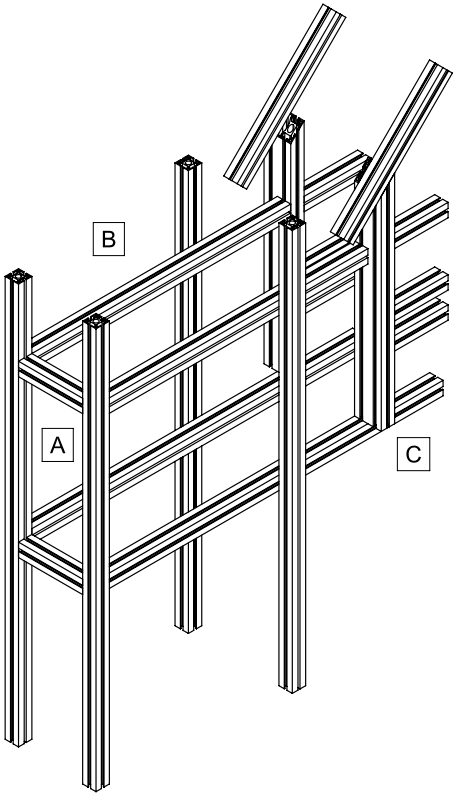
\includegraphics[draft=false,scale=0.41]{Illustrationen/6-Umsetzung/maschinengestell.PNG}
	\caption{Maschinengestell}
	\label{fig:maschinengestell}
\end{wrapfigure}

\textit{(ygu)} Das Maschinengestell basiert auf dem Baukasten System von Kanya AG. Die Profile von Kanya AG eignen sich aus folgenden Gründen:
\begin{itemize}
	\item Dieses System ist einfach im Aufbau und der Montage. Das Maschinengestell ist so aufgebaut, dass eine Anpassung der Höhe (Punkt B in Abbildung \ref{fig:maschinengestell}) und die überstehende Länge der Setzeinheit (C) möglich ist. Diese Flexibilität wird durch die Verwendung der Universallverbinder von Kanya AG möglich.
	
	\item Das Profil hat an jeder Seite eine Längsnut. Dies bietet eine simple Lösung zur Montage der Montagebleche der Setzeinheit sowie Vereinzelung. Zudem ist im hinteren Teil des Gestells (A) eine Aluminiumplatte zur Montage der Elektronik vorgesehen.
	
	\item Die Tatsache, dass die Hochschule Luzern bei Kanya AG bereits Kunde ist, hebt Kanya AG von anderen Konkurrenten ab. Die positiven Erfahrungen und raschen Lieferzeiten überzeugen.
\end{itemize}
Weitere Informationen zum Baukastensystem von Kanya AG ist aus dem Katalog zu entnehmen \cite{kanya}.

\subsubsection{Verdrahtung}
\textit{(pro)} In Abb. \ref{fig:Verdrahtung} ist das Schema der Netzbeschaltung abgebildet. Die Netzspannung des Planting Robots wird aus Sicherheitsgründen über eine Relais Selbsthalteschaltung betrieben welche über den Ein/Aus Taster S1 geschaltet wird. Der Ein/Aus Taster hat eine integrierte Signallampe P1. Als Sicherung dient der Leitungsschutzschalter 5SY4106-7 von Siemens mit 6A Nennstrom.

\begin{figure}[H]
	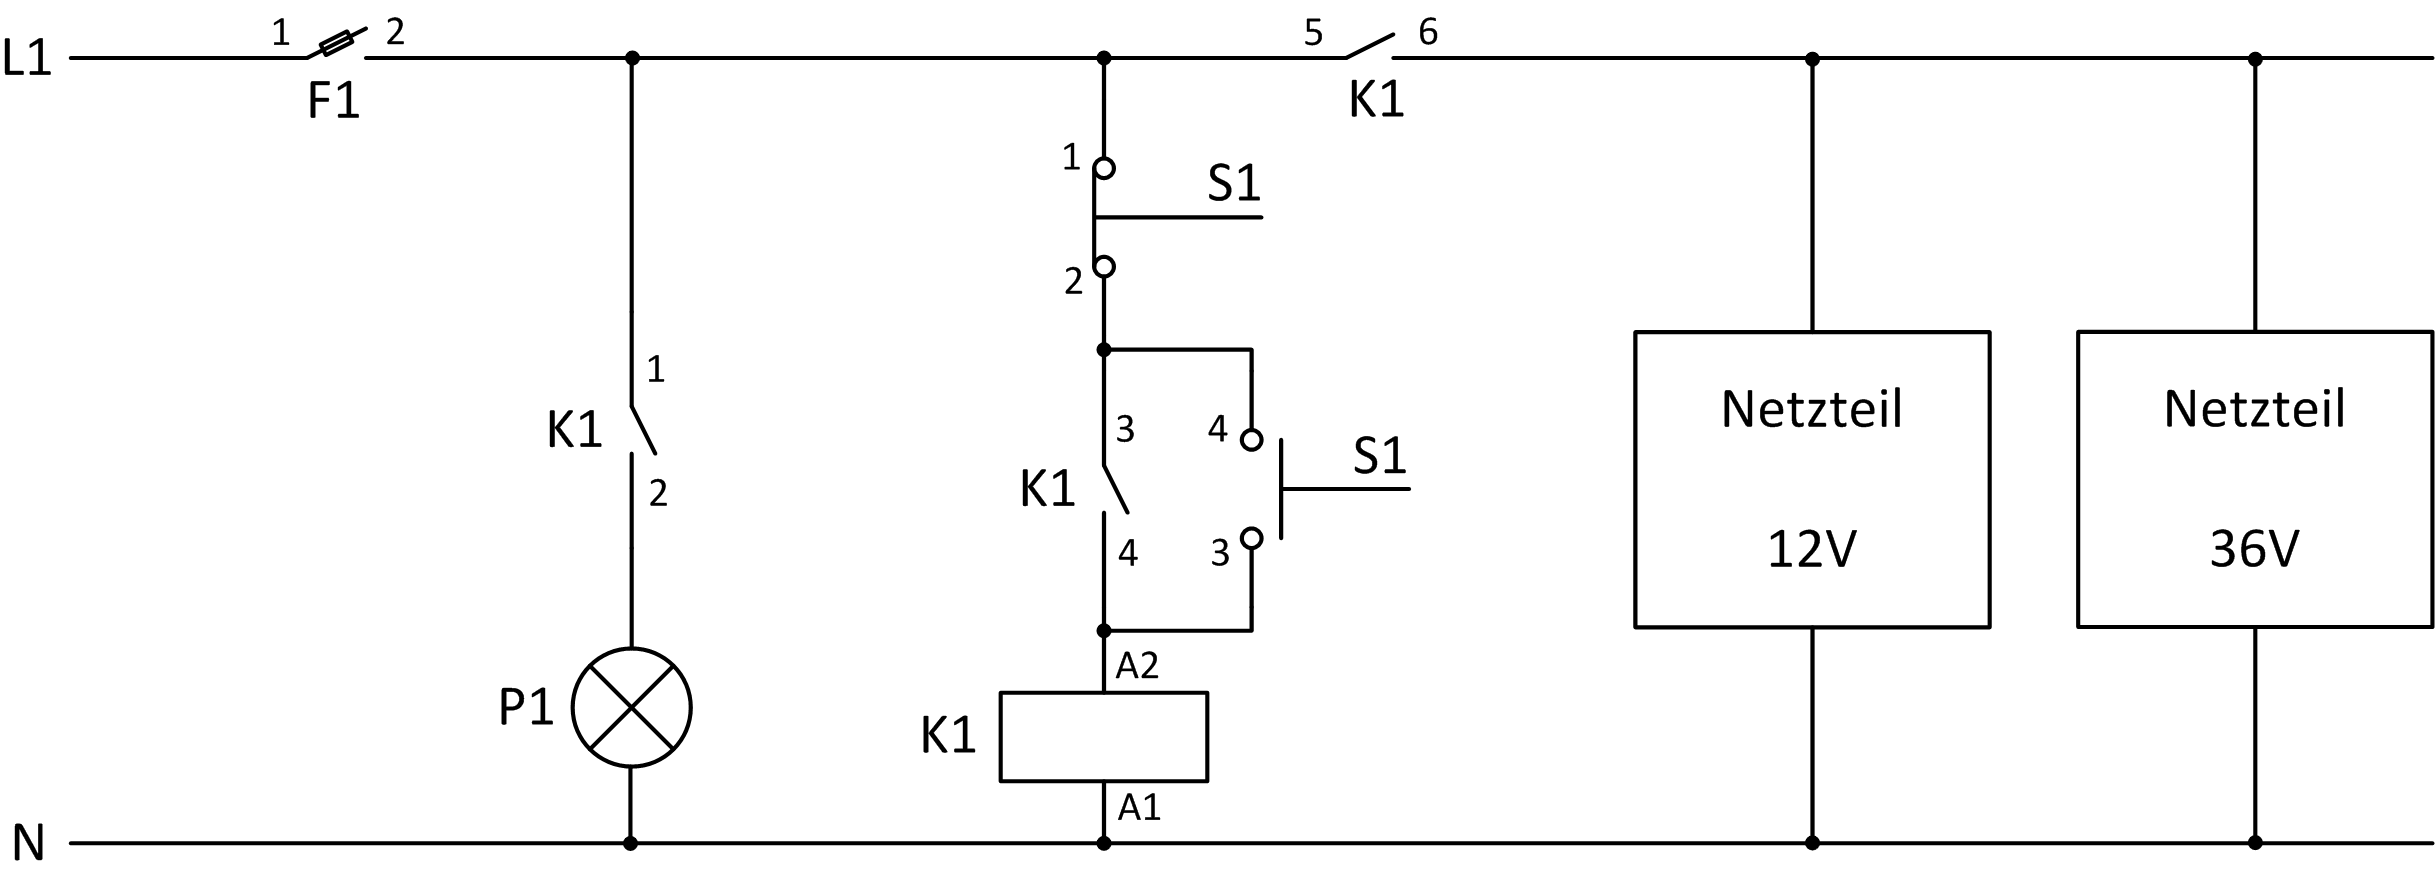
\includegraphics[draft=false,width=0.95\textwidth]{Illustrationen/6-Umsetzung/Verdrahtungsschema.png}
	\caption{Verdrahtungsschema Netzbeschaltung}
	\label{fig:Verdrahtung}
\end{figure}

Die Elektronikkomponenten wurden auf einem Aluminium Blech der Grösse 967mm x 436mm miteinander verdrahtet. Das Blech wurde, wie in Abb. \ref{fig:Schaltschrank} ersichtlich, auf beiden Seiten mit Tragegriffen ausgestattet. Mit Hilfe der Tragegriffe kann die Verdrahtungsanlage einfach transportiert werden. Diese ist vor allem für die Inbetriebnahme von Bedeutung, da die Anlage dadurch nicht an eine bestimmte Räumlichkeit gebunden ist. Die Verdrahtungsplattform wird seitlich in das Maschinengestell eingefahren.

\begin{figure}[H]
	\includegraphics[draft=false,width=1\textwidth]{Illustrationen/6-Umsetzung/Schaltschrank_beschr.png}
	\caption{Verdrahtungsplattform}
	\label{fig:Schaltschrank}
\end{figure}

Die Elektronik Komponenten wurden zur Vorbeugung von EMV Problemen nach Leistungs- und Signalteilen positioniert. So wurde die Netzbeschaltung (in Abb. \ref{fig:Schaltschrank} links unten) mit Distanz zum Mainboard PCB angebracht. Das 36V Netzteil für den BLDC-Motor sowie dessen Motorcontroller wurden nahe beieinander positioniert um kurze Kabel verwenden zu können. Dadurch werden Störungen durch Einkopplung bei parallel geführten Leitungen vermindert.